\section{Agenda}

\begin{frame}
    \begin{itemize}
            \item VPP: A fast Software Router
            \begin{itemize}
                \item Design Goals and Areas of Use
                \item Packet Processing Graph
            \end{itemize}
            \item Tested Scenarios
            \item Benchmarking Setup
            \item Results
            \begin{itemize}
                \item Maximum Throughput: CPU as a Bottleneck
                \item CPU Scaling
                \item Lookup Performance
                \begin{itemize}
                    \item L2
                    \item IPv4 v18.10
                    \item IPv4 v16.04
                    \item IPv6
                \end{itemize}
                \item Latencies
                \item Comparison
            \end{itemize}
            \item Conclusion
        \end{itemize}
\end{frame}

\section{VPP: A fast Software Router}

\begin{frame}
    \frametitle{Design Goals and Areas of Use}
    
    % \begin{figure}
    % 
\includegraphics[width=5cm]{pics/logo_fdio.png}
    % \end{figure}

    % \begin{wrapfigure}
    % 
\includegraphics[width=1in]{pics/logo_fdio.png}
    % \end{wrapfigure}

    \mbox{}\hfill\raisebox{-\height}[0pt][0pt]{
\includegraphics[width=.15\linewidth]{pics/logo_fdio.png}}

    VPP (Vector Packet Processing): 
    \begin{itemize}
        \item software router
        \item user space (DPDK)
        \item mainstream architechtures
    \end{itemize}
    \pause

    Distinctive Features: % differences to other softwarerouters
    \begin{itemize}
        \item open-sourced by Cisco \cite{vppwiki:whatis}
        \item processing graph: feature rich, modular, extensible \cite{linguaglossa2017high}
    \end{itemize}
    \pause

    Use Cases:
    \begin{itemize}
        \item SDN: "foundation of future cloud native services" \cite{florincoras}
        \item Integration into OpenStack \cite{fdio:integration}
        \item VNF: firewalls/DPI \cite{qosmos}\cite{cisco:sdn}
    \end{itemize}

\end{frame}

\begin{frame}
    \frametitle{Packet Processing Graph}

    \begin{itemize}
        \item{dpdk-input: packet vector (max. 256)}
        \item{l2-fwd: BiHash (inline)}
        \item{ip4-lookup: MTree}
        \item{ip6-lookup: BiHash}
    \end{itemize}

    \begin{figure}
    \noindent\hspace{1mm}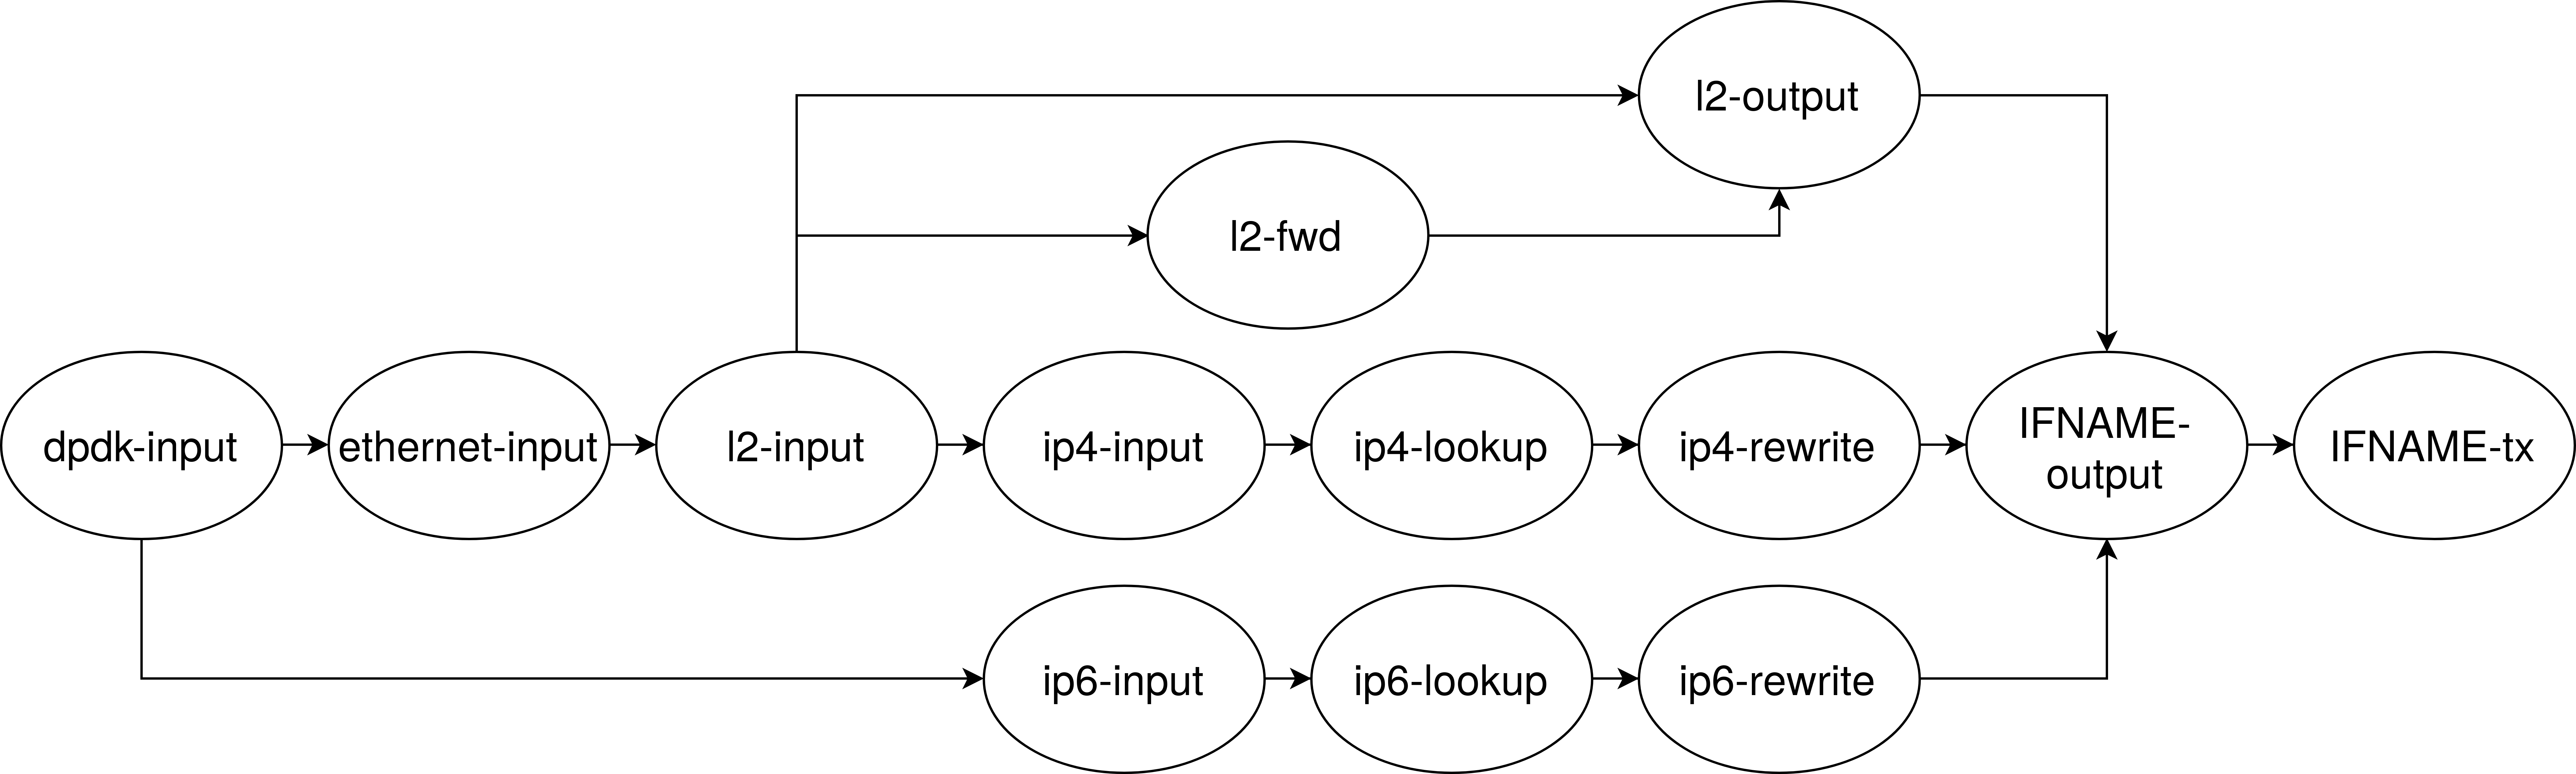
\includegraphics[width=\linewidth]{pics/vpp-nodes-horizontal.png}
    \label{nodegraph}
    \end{figure}
\end{frame}

\section{Tested Scenarios}

\begin{frame}

    Tested Features:
    \begin{itemize}
        \item XConnect
        \item l2 Bridges
        \item l3: IPv4
        \item l3: IPv6
        \item VXLAN
    \end{itemize}

    Tested Parameters: 
    \begin{itemize}
        \item Packet rates
        \item l3 multiple threads and flows
        \item l2/l3 fib sizes
    \end{itemize}

    Hurdles: no l2 multicore, l2 fib filling

    % Implementational and hardware details (why no framesizes): \cite{mywork}

\end{frame}

\section{Benchmarking Setup}

\begin{frame}
    \begin{figure}
    \noindent\hspace{5mm}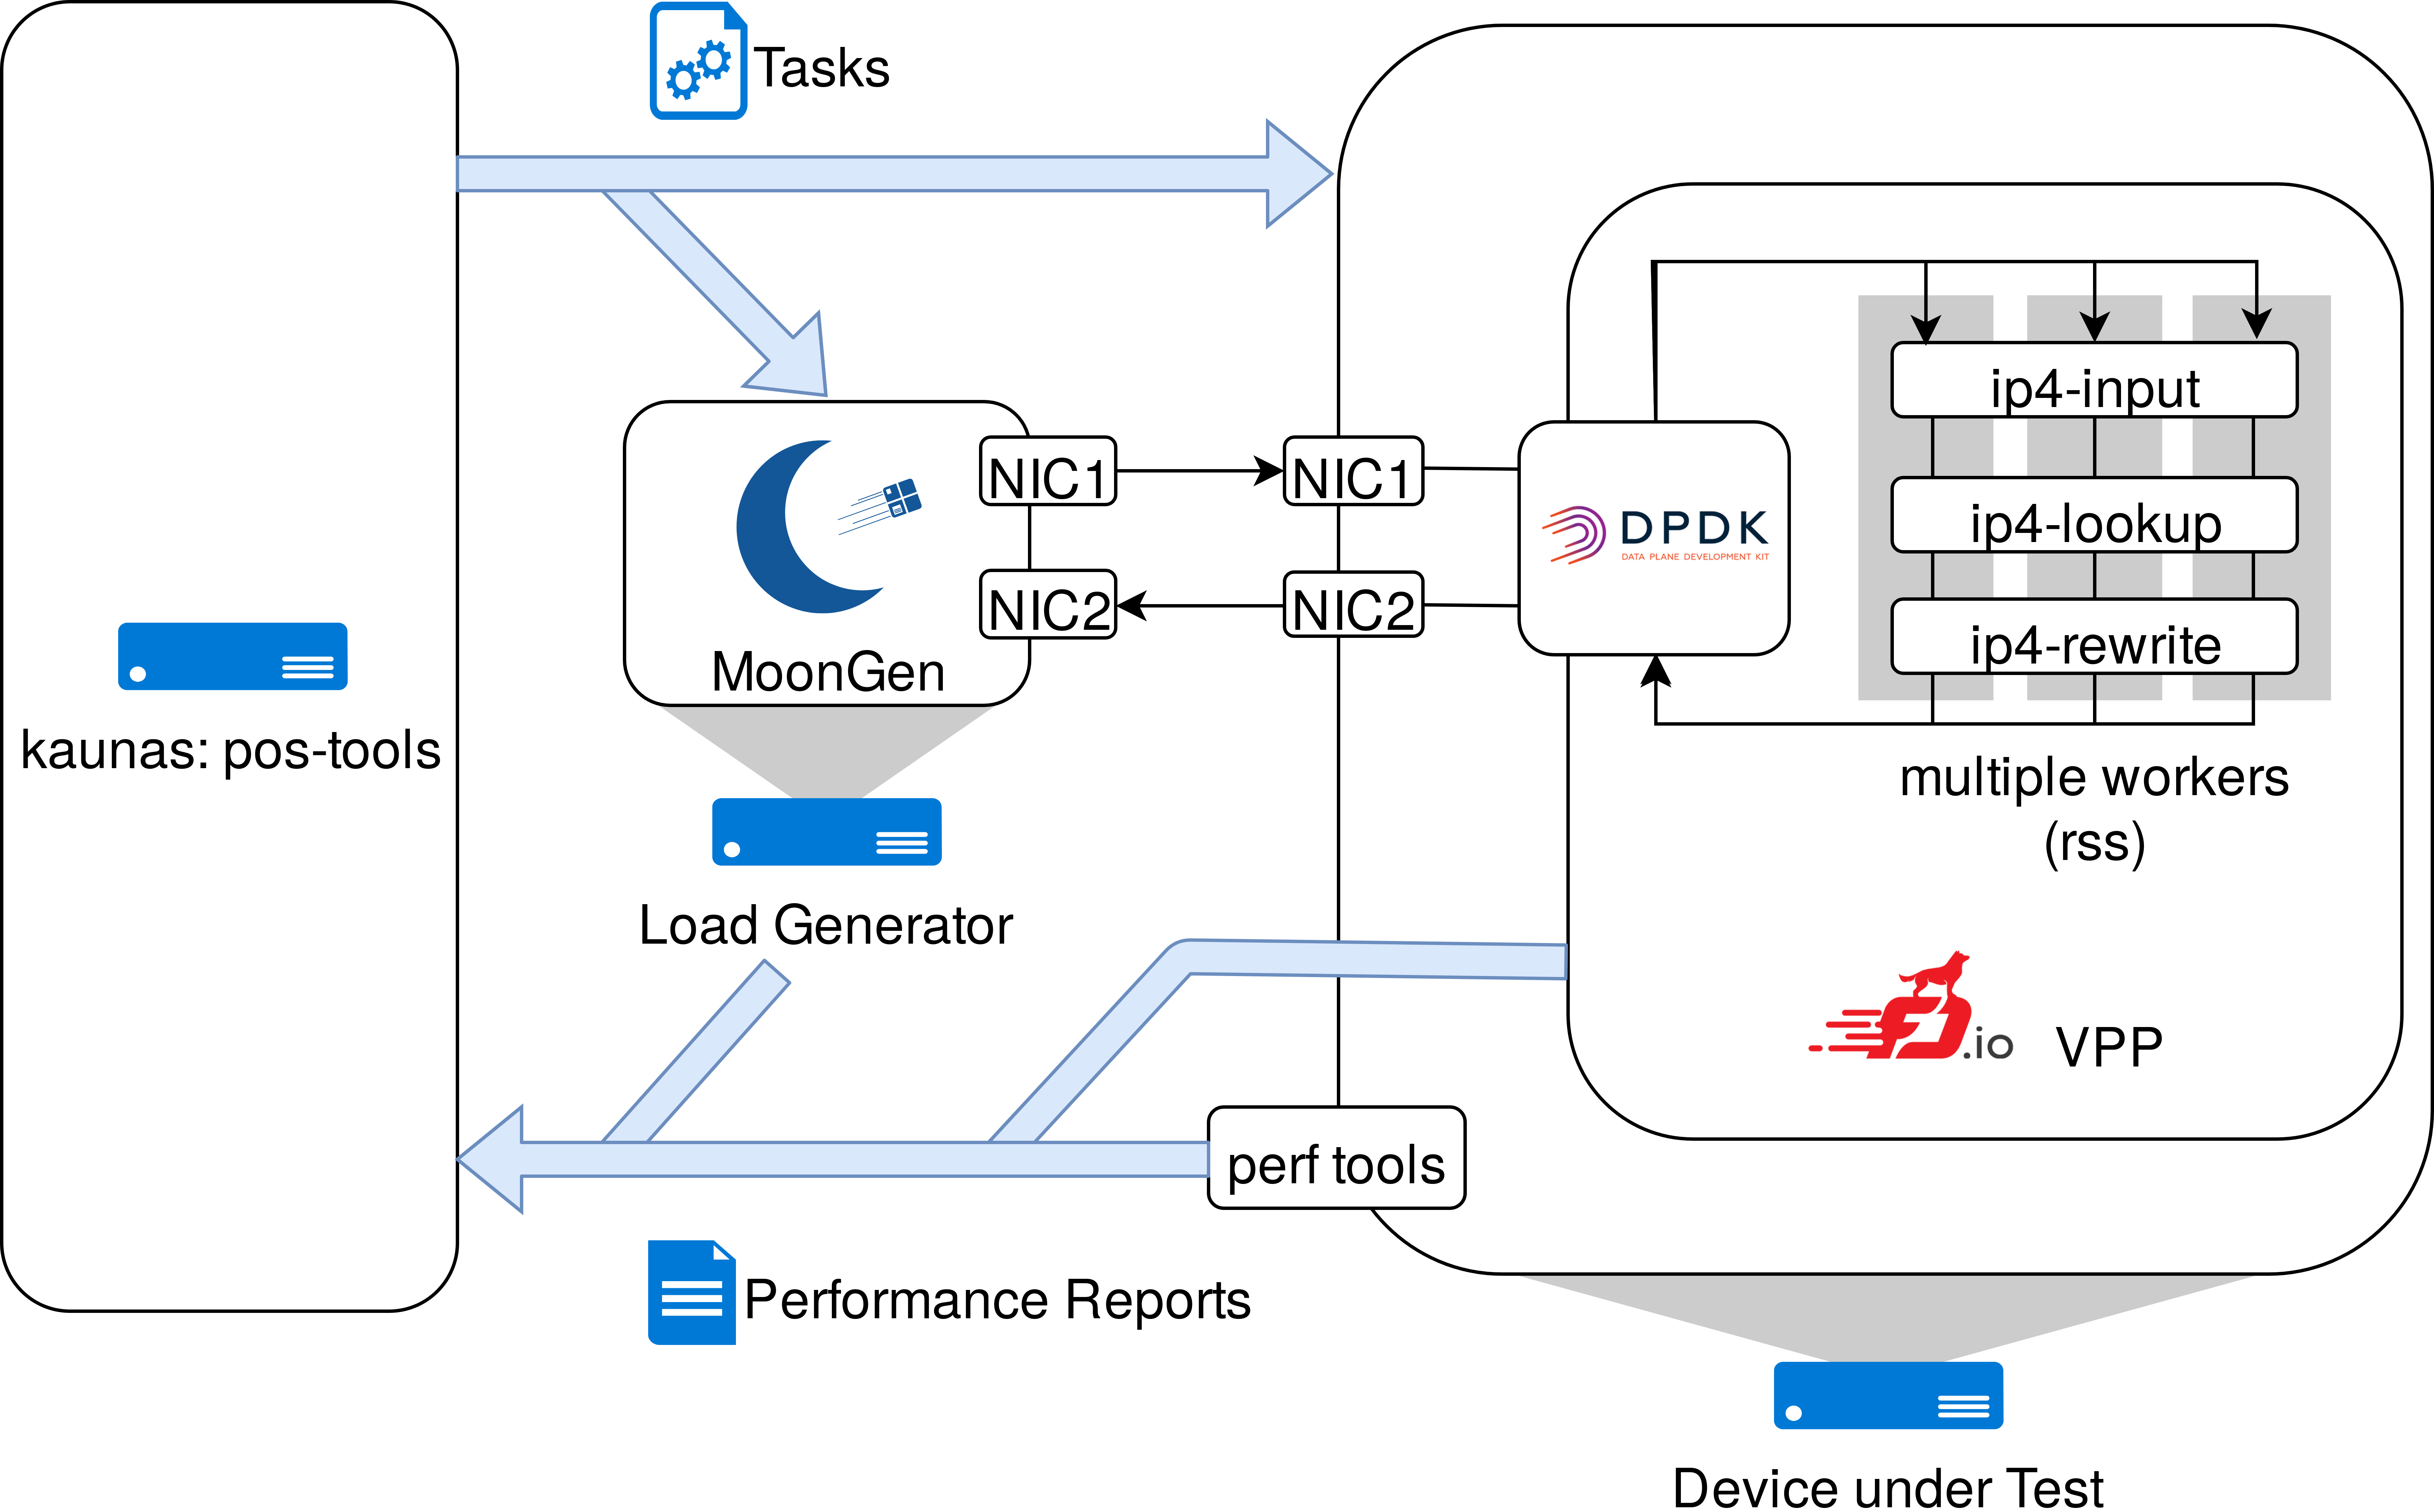
\includegraphics[width=0.9\linewidth]{pics/topology.png}
    %\caption{Experiment setup for testing VPP with "kaunas" management server, LoadGen and DUT}
    \label{setup}
    \end{figure}
\end{frame}


\section{Results: CPU}


\begin{frame}
    \frametitle{Maxumim Throughput: CPU as a Bottleneck}
    \begin{table}[!ht]
        \vspace{5ex}
        \begin{tabular}[]{ l r r r }
            Scenario & 1.6GHz (50\%) & 3.1GHz (97\%)  & 3.2GHz (100\%) \\ 
            \midrule
            xconnect & 7.34 (56\%) & 12.90 (98\%) & 13.20 (100\%) \\ % stdDev 0.03 0.02 0.12
            l2 bridge no features & 6.69 (55\%) & 11.84 (97\%) & 12.18 (100\%) \\ % 0.01 0.03 0.08
            IPv4 1 route & 6.03 (53\%) & 10.98 (97\%) & 11.28 (100\%) \\ % stdDev 0.01 0.02 0.05
            l2 bridge mac-learn, mac-age & 6.05 (55\%) & 10.84 (98\%) & 11.09 (100\%) \\ % 0.01 0.05 0.02
            IPv6 1 route & 5.38 (53\%) & 9.87 (97\%) & 10.14 (100\%) \\ % 0.01 0.02 0.04
            VXLAN encap & 4.48 (55\%) & 8.15 (99\%) & 8.21 (100\%) \\ % 0.01 0.03 0.39
            IPv4 255k routes & 4.19 (58\%) & 7.06 (97\%) & 7.25 (100\%) \\ % 0.01 0.04 0.07
            IPv6 255k routes & 2.34 (62\%) & 3.72 (98\%) & 3.80 (100\%) \\ % 0.01 0.04 0.02
            \midrule
        \end{tabular}
        \label{bottleneck}
    \end{table}
    % With offered Mpps beeing 100\%, "Relative" is the maximum packet throughput in relation to the offered one.
\end{frame}

\begin{frame}
    \frametitle{CPU Scaling}
    \begin{figure}[!ht]
    \noindent\hspace{0.5mm}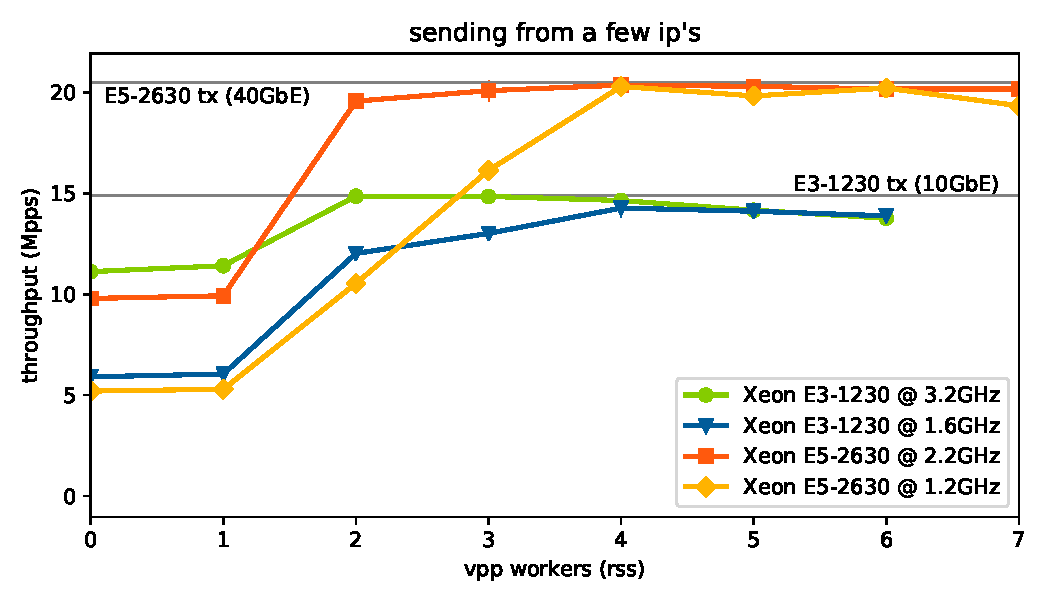
\includegraphics[width=\linewidth]{pics/throughput_summary_multicore.pdf}
    \caption{VPP CPU scaling with IPv4 traffic with 10GbE, 40GbE and different CPU clock speeds. All workers (besides E3-1230 core 3-6) use physical CPU cores. The 40GbE NIC bottlenecks at around 20Mpps (see Section \ref{sec:40gbelimit}). }
    \label{graph:multicore}
    \end{figure}
\end{frame}

\section{Results: Lookup Performance}

\begin{frame}
    \frametitle{L2 FIB}
    \begin{figure}[!ht]
    \noindent\hspace{0.5mm}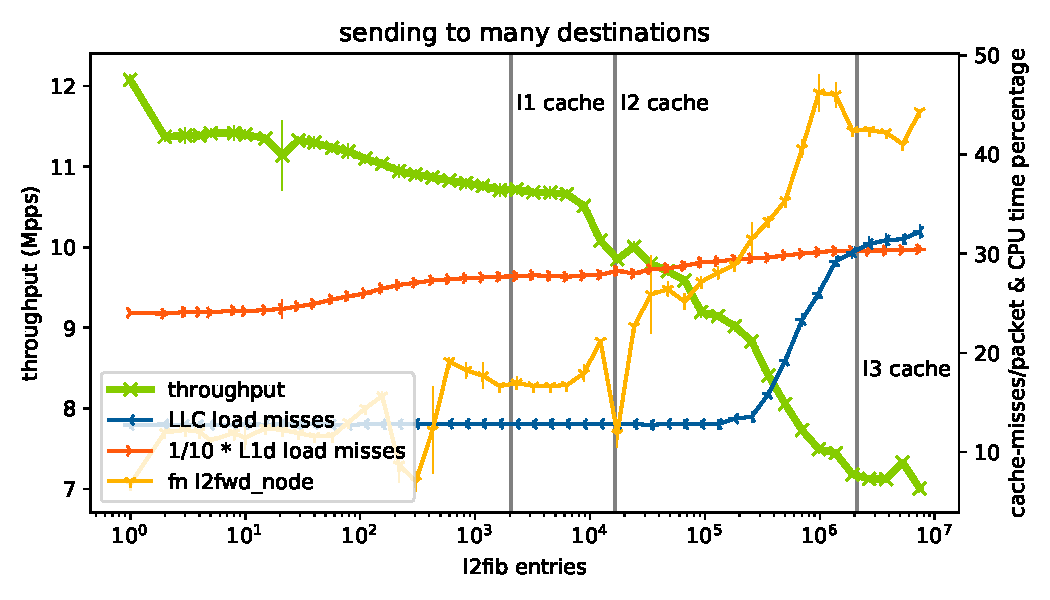
\includegraphics[width=\linewidth]{pics/throughput_l2_throughmac_klaipeda32ghz_v3.pdf}
    \caption{Testing VPP v18.10 with different layer 2 FIB sizes. Throughput, Layer 1 data cache load misses (divided by 10) and Last Level Cache load misses per packet and the percentage of CPU time spent in selected functions. }
    \label{graph:l2fib}
    \end{figure}
\end{frame}

\begin{frame}
    \frametitle{IPv6 FIB}
    \begin{figure}[!ht]
    \noindent\hspace{0.5mm}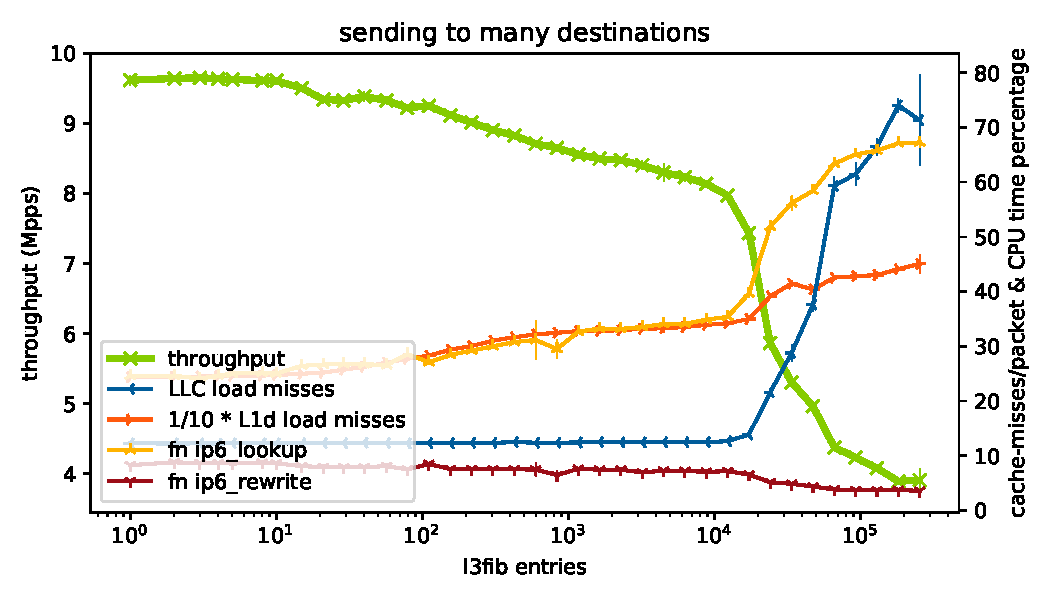
\includegraphics[width=\linewidth]{pics/throughput_l3v6_routes_klaipeda32ghz_v3.pdf}
    \caption{Testing VPP v18.10 with different IPv6 FIB sizes. Throughput, Layer 1 data cache load misses (divided by 10) and Last Level Cache load misses per packet and the percentage of CPU time spent in selected functions. }
    \label{graph:ip6fib}
    \end{figure}
    Lookup nodes as bottleneck
\end{frame}

\begin{frame}
    \frametitle{IPv4 FIB v18.10}
    \begin{figure}[!ht]
    \noindent\hspace{0.5mm}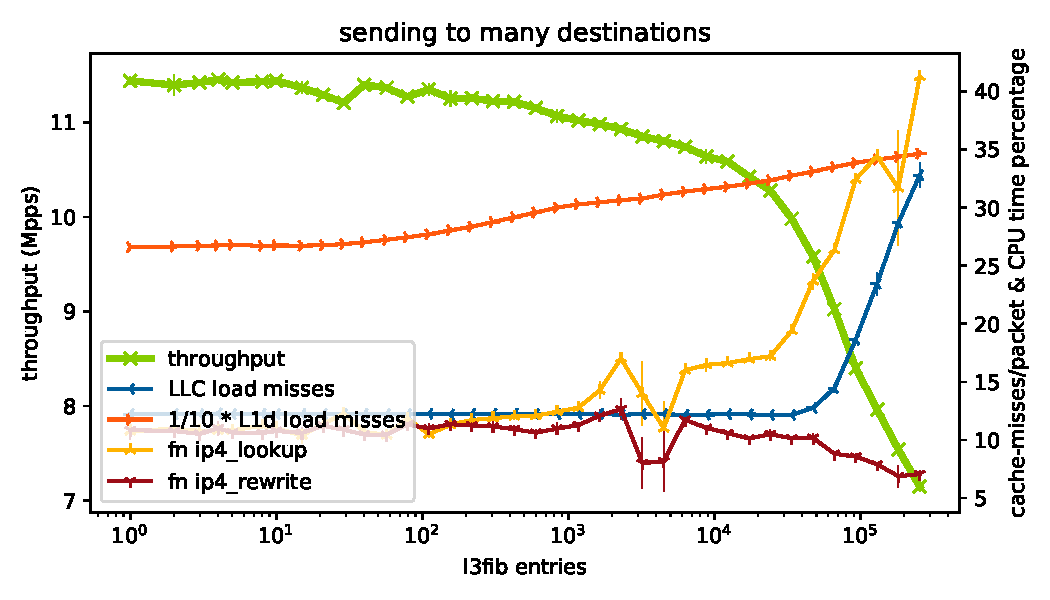
\includegraphics[width=\linewidth]{pics/throughput_l3_routes_klaipeda32ghz_v3.pdf}
    \caption{Testing VPP v18.10 with different IPv4 FIB sizes. Throughput, Layer 1 data cache load misses (divided by 10) and Last Level Cache load misses per packet and the percentage of CPU time spent in selected functions.}
    \label{graph:ip4fib}
    \end{figure}
\end{frame}

\begin{frame}
    \frametitle{IPv4 FIB v16.09}
    \begin{figure}[!ht]
    \noindent\hspace{0.5mm}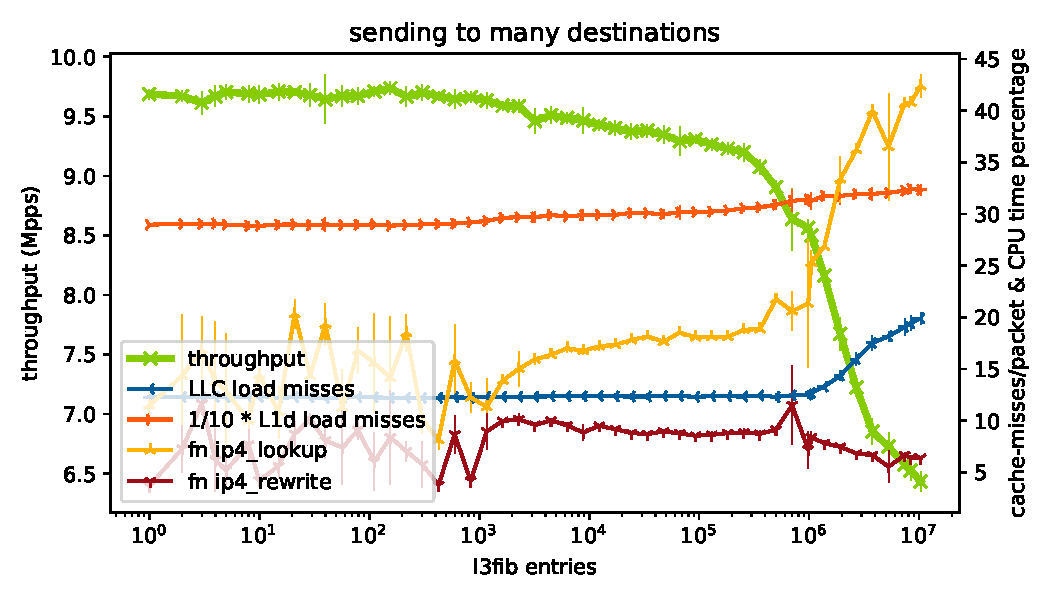
\includegraphics[width=\linewidth]{pics/throughput_l3_routes_klaipeda_v1609_32ghz_v3.pdf}
    \caption{Testing VPP v16.09 with different IPv4 FIB sizes. Throughput, Layer 1 data cache load misses (divided by 10) and Last Level Cache load misses per packet and the percentage of CPU time spent in selected functions. }
    \label{graph:ip4fiblegacy}
    \end{figure}
\end{frame}

\section{Results: Latencies}

\begin{frame}
    \frametitle{asdad}
    \begin{figure}[!ht]
    \noindent\hspace{0.5mm}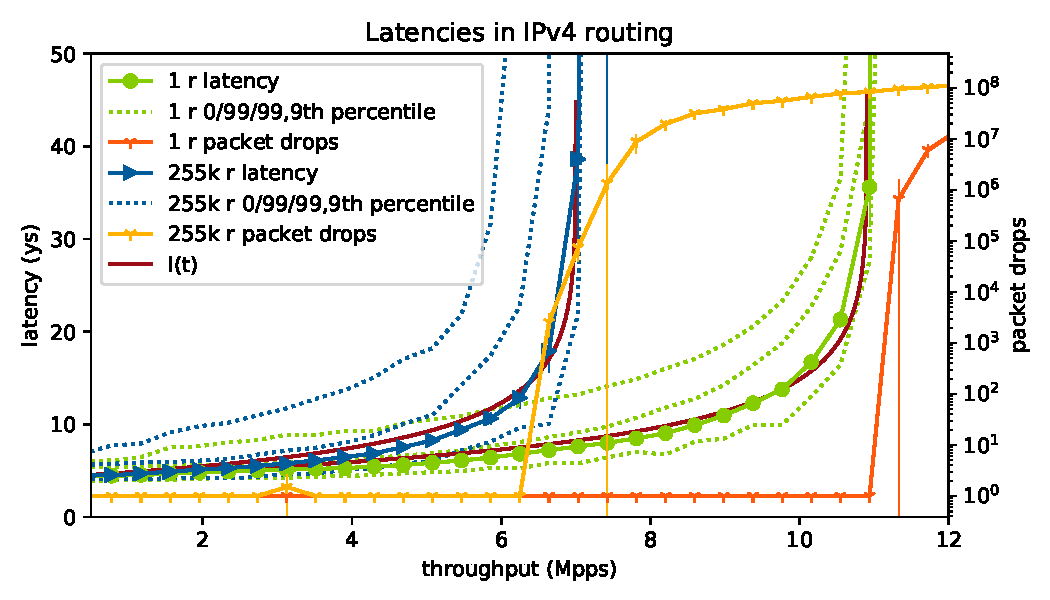
\includegraphics[width=\linewidth]{pics/latencies_per_throughput_summary_ip4.pdf}
    \caption{Latencies in $\mu s$ and packet drops of IPv4 routing with a single route (1 r) and 255k routes (255k r). }
    \label{graph:latencyoverview}
    \end{figure}
\end{frame}

\begin{frame}
    \frametitle{Histogram}
    \begin{figure}[!ht]
    \noindent\hspace{0.5mm}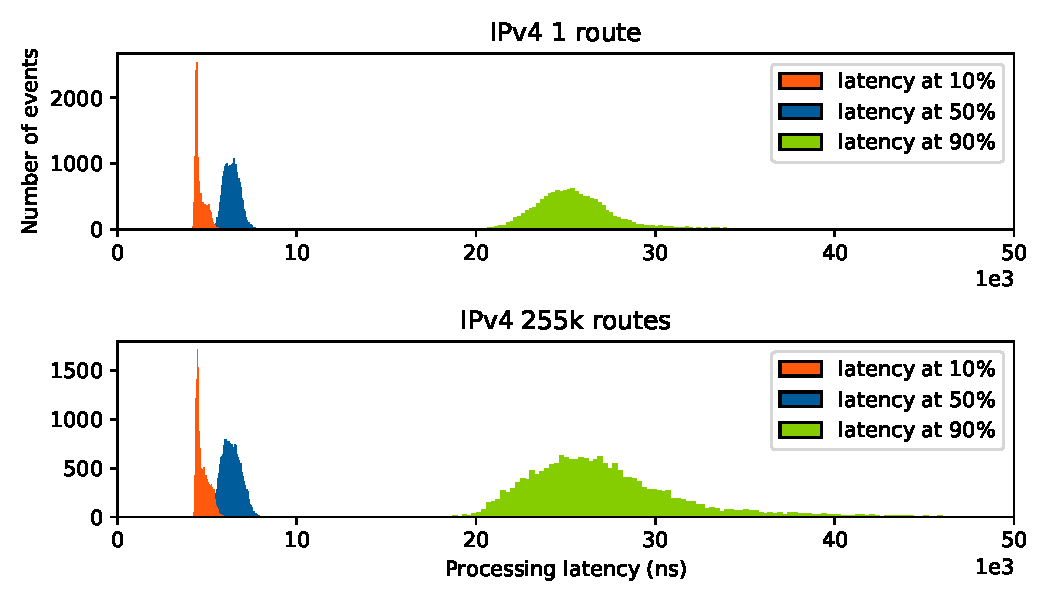
\includegraphics[width=\linewidth]{pics/latency_histogram_overview_ip4.pdf}
    \caption{Latency histogram for IPv4 routing with a single route and 255k routes at approximately 10\%, 50\% and 90\% of the maximum throughput rate. }
    \label{graph:latencyhistogram}
    \end{figure}
\end{frame}

\section{Results}


\begin{frame}
    \frametitle{Comparison}
    % TODO graphical visualization
    \begin{table}
        \begin{tabular}[]{ l r r r }
            Implementation   & FIB sizes & Mpps     & Relative \\ 
            \midrule
            MoonRoute        & 1         & 14.6     & 100\% \\
            MoonRoute        & $2^{20}$  & 14.2     & 97\% \\
            MoonRoute        & $2^{24}$  & 11.6     & 79\% \\
            VPP v18.10       & 1         & 11.6     & 79\% \\
            FastClick DPDK   & 1         & 10.4     & 72\% \\
            FastClick DPDK   & $2^{20}$  & 10.4     & 72\% \\
            VPP v16.09       & 1         & 9.7      & 71\% \\
            VPP v16.09       & 255k      & 9.2      & 63\% \\
            VPP v16.09       & $2^{20}$  & 8.5      & 58\% \\
            VPP v18.10       & 255k      & 7.2      & 50\% \\
            VPP v16.09       & $2^{23}$  & 6.5      & 45\% \\
            Click DPDK       & 1         & 4.3      & 29\% \\
            Click DPDK       & $2^{20}$  & 4.2      & 28\% \\
            Linux 3.7        & 1         & 1.5      & 11\% \\

            \midrule
        \end{tabular}
        \caption{Comparison of maximum IPv4 forwarding throughput with a single worker on the Xeon E3-1230 system. Non-VPP results are from \cite{chair:architecture} and are conducted on the same system. }
        \label{table:comparison}
    \end{table}
\end{frame}

\section{Conclusion}

\begin{frame}
asdsad
\end{frame}


\section{Questions?}

\begin{frame}
    \frametitle{Example frame}
    \begin{itemize}
        \item item 1
        \item $\ldots$
        \begin{itemize}
            \item test
            \item $\ldots$
        \end{itemize}
    \end{itemize}
    Citation \cite{rfc959}

    \paragraph{Math mode should be fully functional:}
    $$
    \hat s
    \overline s
    \mathcal S
    \mathbit S
    \mathbit \Lambda
    \sum
    \pd{\xi}
    \pr{X=0}
    \mathbit 1
    $$
\end{frame}

\begin{frame}
    \frametitle{Figures}
    \begin{figure}
        \centering
        \includegraphics[width=.5\textwidth]{figures/example}
        \caption{Figure caption}
        \label{Maizaso0}
    \end{figure}
    Figure~\ref{Maizaso0} shows a small network.
\end{frame}

\begin{frame}
    \frametitle{Figures}
    \begin{table}
        \begin{tabular}{rccc}
            \toprule
            & Competitor 1 & Competitor 2 & we\\
            \midrule
            Feature A & \no & \maybe & \yes\\
            Feature B & \no & \maybe & \yes\\
            Feature C & \no & \maybe & \yes\\
            Feature D & \no & \maybe & \yes\\
            \bottomrule
        \end{tabular}
    \end{table}
\end{frame}

